\section{Zusammenhang HTTP(s) und Zertifikate}
\label{sec:HTTPs}
Der Nutzer besucht z. B. eine Onlinebanking Webseite, die durch das Kürzel HTTPS signalisiert, dass es sich um eine verschlüsselte Verbindung handelt. Bei jeder HTTPS-Kommunikation muss sich der Webserver, auf dem die Internetseite gehostet wird, authentifizieren. Die Authentifizierung des Webservers gegenüber des Clients erfolgt durch ein für den Webserver ausgestelltes Zertifikat. 
Das Zertifikat enthält unter anderem den öffentlichen Schlüssel (Public Key), einen eindeutigen Fingerabdruck und Angaben über den Zertifikatsinhaber. Ein Zertifikat verbindet somit einen Inhaber mit einem öffentlichen Schlüssel. Mit dem Public Key verschlüsselt der Client die Daten, die er zum Webserver schickt. Anhand des Fingerabdrucks, welcher auch als digitale Signatur des Zertifikats bezeichnet wird, überprüft der Client, ob er mit dem richtigen Webserver kommuniziert. Der Fingerabdruck wird durch einen Hashalgorithmus wie z. B. SHA-2 erzeugt. Bei der Erzeugung gehen diverse Daten wie z. B. Zertifikatsaussteller, öffentlicher Schlüssel und Identifizierungsdaten über den Webserver mit ein. 
Wenn das Zertifikat von einer Zertifizierungsstelle (Certification Authority = CA) ausgestellt wurde, deren eigenes Zertifikat (= Root-Zertifikat oder Wurzelzertifikat) bereits im Browser installiert ist, dann wird dem ausgestellten Zertifikat automatisch vertraut. In den bekanntesten Webbrowsern wie z. B. Firefox, Chrome oder der Internet Explorer sind bereits viele Root-Zertifikate von den weltweit verschiedenen Zertifizierungsstellen vorinstalliert.
\begin{figure}[H]
		\centering
		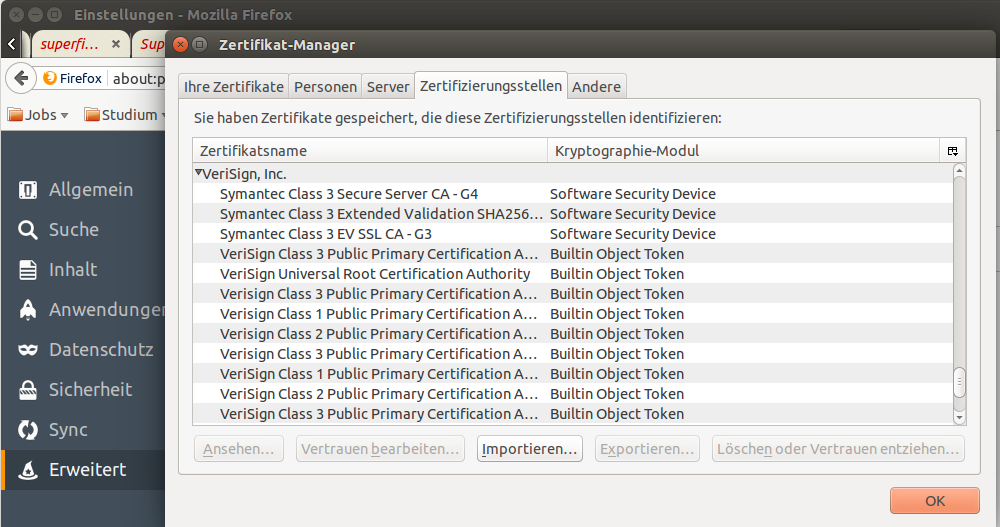
\includegraphics[width=1\linewidth]{images/firefox_installierte_zertifikate.png}
		\caption{Ausschnitt vorinstallierter Zertifikate im Firefox Browser}
\end{figure}
\noindent
Nutzt der Webservers jedoch ein selbst ausgestelltes (selbst signiertes) Zertifikat zur Authentifizierung, dann wird beim Verbindungsaufbau dem Nutzer eine Warnung angezeigt (siehe Bild ...). Der Nutzer kann anschließend selbst entscheiden ob er dem Zertifikat vertraut oder nicht. Außerdem entscheidet er ob er nur ein einziges Mal, d. h. nur für diese Verbindungssession, dem Zertifikat vertraut oder ob er eine dauerhafte Ausnahme macht. Ist letzteres der Fall, dann wird das Zertifikat im Browser installiert. Es wird dann bei den schon vorinstallierten Zertifikaten mit abgelegt. Eine dauerhafte Ausnahme hat zu Folge, dass der Benutzer beim Verbindungsaufbau zu der zugehörigen Webseite vom Webbrowser nicht mehr gewarnt wird. 